\section{Methodology}
This section presents the procedures for developing a Scalable Decentralized Cooperative Platoon (SDCP). Connected autonomous vehicles are trained together to learn how to drive on a track with turns and obstacles while learning how to drive in a platoon formation and respect its regulations like keeping the same gap between vehicles and the same velocity as the predecessor vehicle. Figure 1 shows the proposed Markov Decision Process (MDP) for this multi-agent reinforcement learning problem. MDP framework supports formalizing the loop between the agents and the environment \cite{littman1994markov}; agents interact with the environment by taking actions that result in a new state with feedback from the environment in the shape of rewards that gives a clue to the learning behavior's action whether it is a good or bad decision. SDCP should be able to maximize the performance of this cooperative task, platoon formation, and each agent/vehicle's single performance. The environment is developed to help agents learn this behavior to be greedy for maximizing rewards from solo driving and cooperative driving.

\begin{figure}[H]
    \centering
    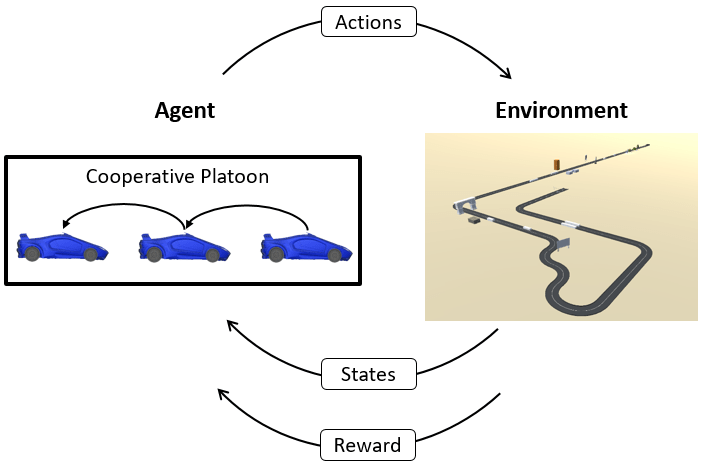
\includegraphics[scale=0.35]{Figures/mdp5-min.PNG}
    \caption{MDP for SDCP}
\end{figure}


\subsection{Environment}
The work is conducted in an urban environment with certain rules, such as vehicles driving on the right lane, no crashes, and car-following driving behavior. Track structure, checkpoints, and obstacles form the environment, as shown in Figure 2, which the agents will interact with. Environment corresponds to agents' actions by sending back positive or negative rewards based on the taken action and presenting new situations to the agents. With these interactions, vehicles learn to drive autonomously while maintaining safe driving and respecting platoon formation.

\begin{figure}[H]
    \centering
    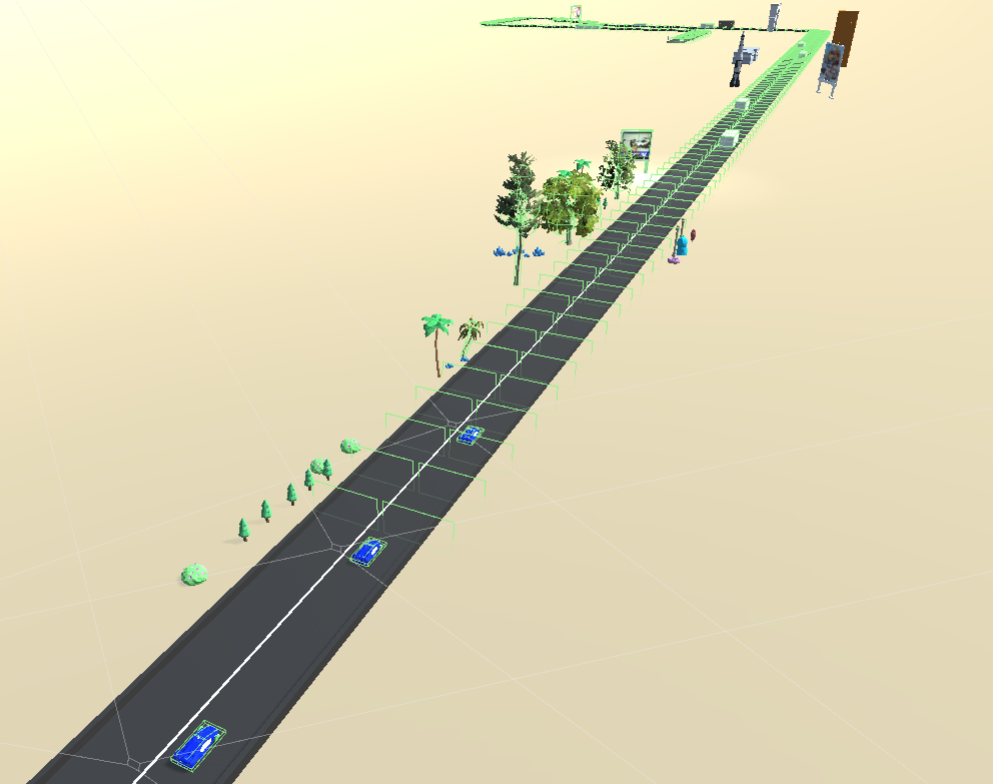
\includegraphics[scale=0.35]{Figures/Env25.PNG}
    \caption{Training Environment}
    \label{fig:my_label}
\end{figure}

\subsubsection{Track Design}
The track is designed to scale up the complexity of driving scenarios. First, vehicles learn to drive on a straight long highway road on the right lane while avoiding hitting road borders or other vehicles, then complexity increases by avoiding crashing static obstacles, and then by driving through complex turns.

\subsubsection{Checkpoints}
Right and left lanes are full of checkpoints, invisible non-rigid colliders, as shown in Figure 3, which guide vehicles through rewards to learn that they should drive in the right lane unless to avoid crashing, which will result in higher negative reward than to do lane change and drive on the left lane.

\begin{figure}[H]
    \centering
    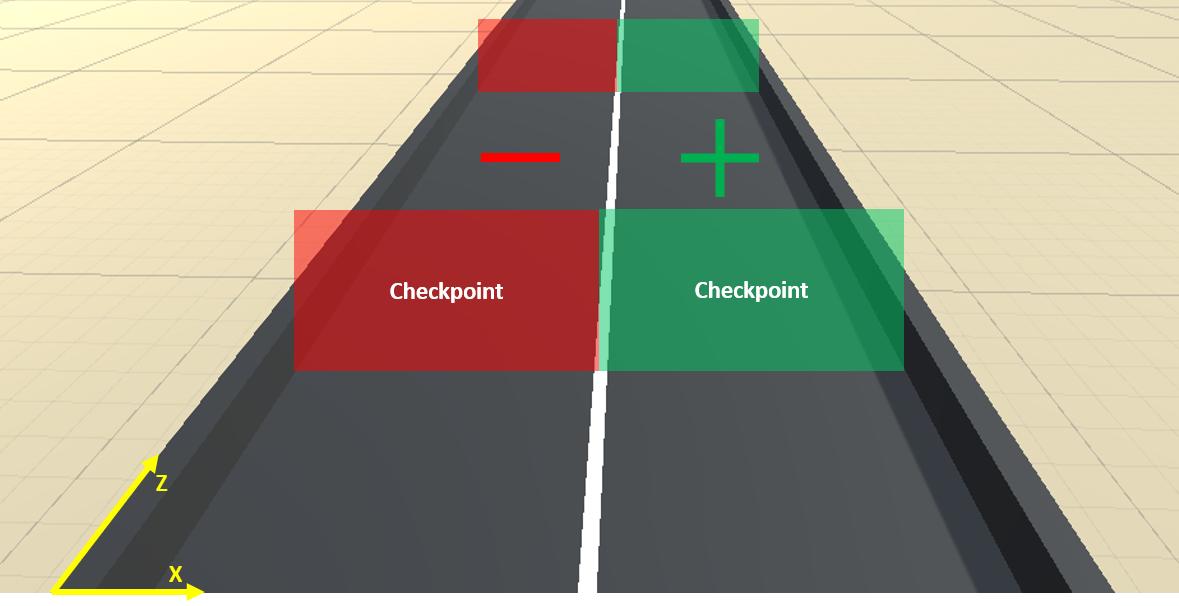
\includegraphics[scale=0.35]{Figures/ckpt1.PNG}
    \caption{Checkpoints}
\end{figure}



\subsubsection{Obstacles}
There are two types of obstacles. Static obstacles, which are rigid solid boxes, represent a scenario of a stopped vehicle, closed road, or an obstacle that would force vehicles to do lane change.
Dynamic obstacles are the other vehicles in the platoon.


\subsection{Multi-Agent}
Three vehicles are connected and trained using model-free Deep RL, where model-free RL is a powerful general tool for learning complex behaviors \cite{pong2018temporal}, to learn how to drive on the track while focusing on safe driving, by avoiding crashing with track borders, static obstacles, or dynamic obstacles (other vehicles).
The developed vehicle dynamical model by Unity \cite{UnitySA} is used in this work to have a highly accurate and realistic dynamic model that quite matches real-life physics.

\begin{figure}[H]
    \centering
    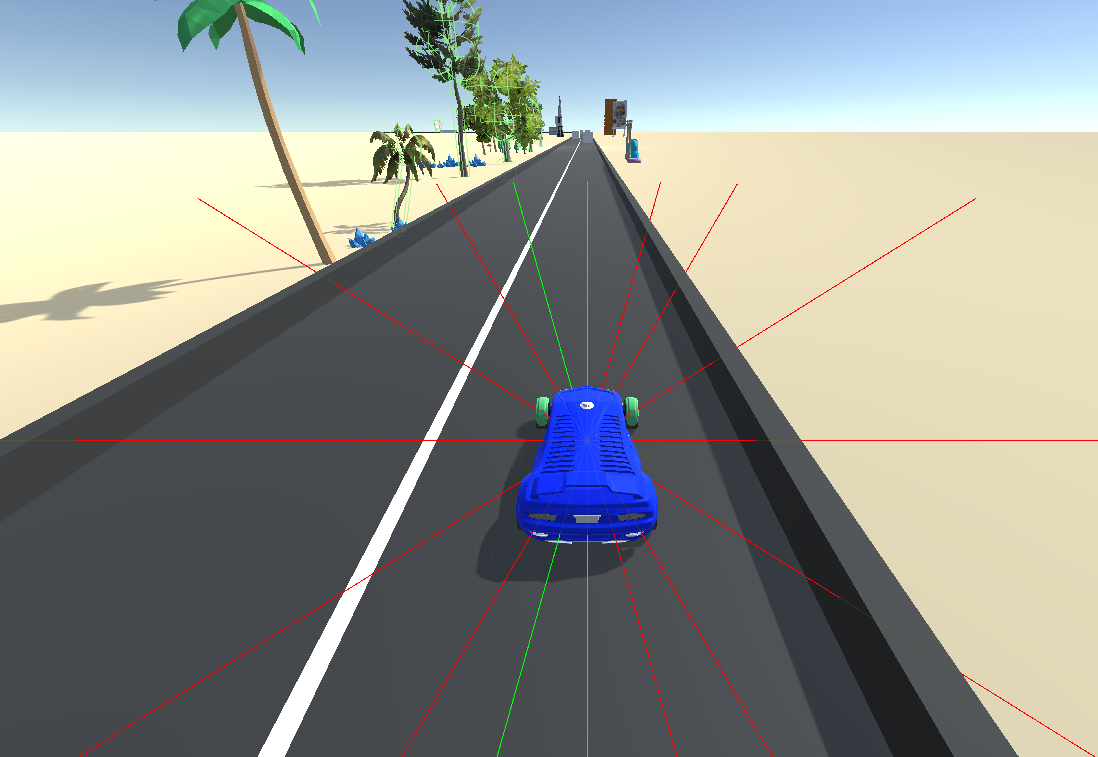
\includegraphics[scale=0.375]{Figures/Car29.PNG}
    \caption{Agent/Vehicle}
    \label{fig:my_label}
\end{figure}

\textbf{Ego Perception}
The vehicle needs to observe the surrounding environment to learn how to drive. These observations are also the inputs to the deep neural network of the training model. The vehicle's perception consists of 16 raycast sensors, in which each raycast is like a depth sensor that measures the distance to the facing objects within its range of measuring as visualized in Figure 4, the vehicle's velocity, the gap between it and the predecessor vehicle and the shared data through V2V communication.

\subsection{Scalable Decentralized Cooperative Platoon (SDCP)}
SDCP's foundational principles include V2V communication, decentralization, and scalability. V2V communication forms the backbone of the cooperation, facilitating the seamless exchange of data between the AVs, which is essential for coordinating movements and ensuring safety. Decentralization plays a crucial role, as it allows each vehicle to operate autonomously and make decisions independently, enhancing the system's resilience and flexibility. This decentralization is crucial in scenarios where the lead vehicle may encounter issues, allowing for quick reorganization without compromising the platoon's functionality. Lastly, scalability is a key principle, ensuring that the system can efficiently adapt to varying sizes of the vehicle platoon without a significant impact on performance or safety. This scalability is vital for accommodating different traffic conditions and platoon configurations, making the SDCP a robust solution for a wide range of real-world applications.\\
In practice, both leader and follower vehicles operate without prior knowledge of road layouts or obstacles, focusing on safe navigation. Safety is the paramount concern, even more so than maintaining platoon formation. For example, if the platoon leader is involved in an accident, the system adapts by reassigning the lead role to the first follower, ensuring both continuity and safety. The leader vehicle prioritizes safe driving, not collecting perception data from followers but rather providing its own sensory information to them. This approach maintains formation and avoids risky maneuvers or actions that might lead to accidents or disrupt the platoon's cohesion, demonstrating the SDCP's commitment to safety and efficiency in various real-world scenarios.\\
The below subsections illustrate SDCP core concepts:\\


\subsubsection{Sharing and Caring Communication Topology}
V2V communication utilizes a predecessor-follower topology, chosen for its minimal impact on computational load as the number of vehicles in a platoon increases. Although alternate topologies may offer superior control, the predecessor-follower system is being refined to enhance platoon scalability and high driving performance without encountering big data challenges \cite{zheng2014influence}. This refinement is influenced by the "sharing and caring" concept, as originated and described by this study \cite{abdelrahman2023development}, which boosts the cooperation between connected AVs. The "sharing and caring" concept is set to be integrated into the predecessor-follower communication topology to foster cohesive cooperation among connected autonomous vehicles.
Through this improved protocol, AVs not only focus on their performance but also consider the welfare and performance of others in the platoon. This enhances cooperation as vehicles share key data like raycast sensor readings and velocity. Importantly, before executing any critical maneuvers, vehicles assess the potential impact on the platoon, especially avoiding actions that could lead to accidents. This cooperative approach promotes safer autonomous driving, strengthens the bond between connected vehicles, and increases the collective rewards for all vehicles in the platoon. Figures 5 and 6 in the referenced document visually depict these differences in communication topology among platoon vehicles.

\begin{figure}[H]
    \centering
    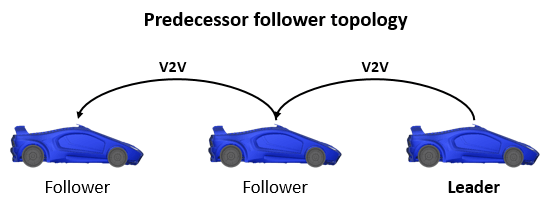
\includegraphics[scale=0.5]{Figures/topology3-min.PNG}
    \caption{Predecessor Follower Communication Topology}
    \label{fig:my_label}
\end{figure}

%Sharing and Caring Communication Topology 
\begin{figure}[H]
    \centering
    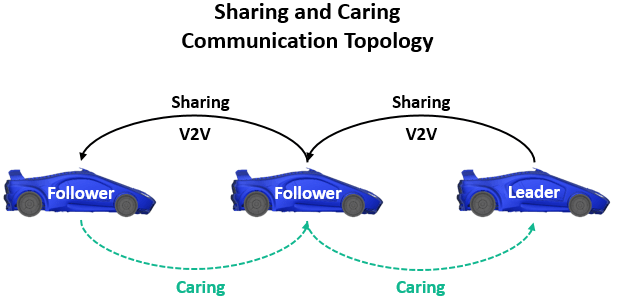
\includegraphics[scale=0.5]{Figures/topology7-min.PNG}
    \caption{Predecessor Follower-based Sharing and Caring Communication Topology}
    \label{fig:my_label}
\end{figure}




\subsubsection{Decentralized Training}
Vehicles are trained together while sharing their data and caring for each other's cumulative rewards based on the developed communication topology, however, each agent is also greedy for its cumulative rewards.
Forcing each agent to focus on maximizing both its rewards and cooperation rewards enables the ability to have both dependent and independent behaviour. The vehicle will depend on other vehicles to gain more rewards from cooperation, but if this cooperation will cause large negative rewards to the agent, it will decide to be independent and focus on driving safely till reaching the desired destination. So for a platoon as an application or form of cooperative driving, vehicles will learn how to drive in a group and respect the platoon formation while being able to drive safely and solely if needed.


\subsubsection{Scalability}
The above-mentioned concepts (sharing and caring communication topology and decentralization) made it applicable to have a scalable number of vehicles in a platoon. It is like a chain where platoon length can be increased or decreased starting from a platoon consisting of a single vehicle to n-number of vehicles as long as this length can fit into the road design and structure.


\subsection{RL Reward Signals}
Reward shaping is a very critical aspect of RL training performance as it is the way of communication to the agent to evaluate it in order to achieve the required behavior.
Curriculum Learning\cite{bengio2009curriculum} is applied on penalties like those caused by crashes to let vehicles have the courage to train with fewer worries about negative rewards at the beginning of training and then penalties' values are increased to give higher priority to safe driving and avoid any crashes or platoon dissociation. If penalties are high from the start of training, sometimes agents decide to stop driving or are afraid of taking any action that may lead to high negative rewards and this slows down the training progress and may lead to passive, not active behavior.

All vehicles in the platoon are subjected to the same positive rewards as shown in Table I, which are the reward signals that focus on teaching vehicles that they should drive in the right lane and as fast as possible to collect more positive rewards. Penalties or negative rewards are the reward signals that teach vehicles safe driving (avoid crashing with track borders, obstacles, or other vehicles). These numerical values for reward signals are subjected based on a trial and error method.
Table I presents rewards for only the discrete events, while speed and gap error penalties are subjected to each time step.

\begin{table}[H]
\centering
\caption{Reward Signals for Discrete Events} 
\resizebox{8.5cm}{!}{
\renewcommand{\arraystretch}{1.5}
\begin{tabular} {|c||c|c|c|} 
 \hline
 \textbf{Event} & \textbf{Reward [0-10m]} & \textbf{Reward [10-15m]} & \textbf{Reward [15-25m]}\\
 \hline
 Checkpoints of right lane & +1 & +1 & +1\\
 \hline
 Checkpoints of left lane & -0.1 & -1 & -2\\
\hline
Reach finish line & +100 & +100 & +100\\
\hline
Follower vehicle reaches finish line & +50 (caring) & +50 (caring) & +50 (caring)\\
\hline
Crash & -10 (no caring) & -10 (no caring) & -50 (no caring)\\
\hline
\end{tabular} }
\end{table}

To apply caring between agents, agents should learn that working cooperatively results in positive rewards, and not helping each other results in negative rewards. Each follower vehicle in the platoon cares about the predecessor vehicle and this is applied by giving a positive reward to the predecessor vehicle if the follower reaches the finish line and a negative reward in case of crashes. This trains the predecessor vehicle to avoid any aggressive actions that may lead to crashes or disorder behavior among the platoon.

The formulated penalty equation of velocity error for the leader:
\begin{gather}
e_{velocity,l} = V_l - V_{desired} \\
P_{velocity,l} = -(e_{velocity,l}/V_{max})^2
\end{gather}  

where $e_{velocity,l}$ is the calculated error between the desired velocity for the platoon and leader vehicle’s velocity, and $P_{velocity,l}$ is the corresponding applied velocity penalty on the leader per stamp time.

Followers are subjected to penalties for gap and velocity errors:

\begin{gather}
e_{velocity,f} = V_f - V_{predecessor} \\
P_{velocity,f} = -(e_{velocity,f}/V_{max})^2\\
e_{gap,f} = G_f - G_{desired}\\
P_{gap,f} = -(e_{gap,f}/G_{max})^2
\end{gather}

where $e_{velocity,f}$ is the velocity error between the follower and predecessor vehicles, $P_{velocity,f}$ is the corresponding applied velocity penalty on the follower vehicle, $e_{gap,f}$ is the measured error in the gap between the follower and predecessor vehicle and $P_{gap,f}$ is the subjected penalty on the follower vehicle for the gap.
The gap ($G_f$) between the ego vehicle’s position ($x_ego$, $z_ego$) and the predecessor vehicle’s position ($x_{predecessor}$, $z_{predecessor}$) is calculated as follows:


where the gap between the ego vehicle and the predecessor vehicle is calculated as follows:
\begin{gather}
G_f = \sqrt{(x_{ego} - x_{pred}) + (z_{ego} - z_{pred})}
\end{gather}

Velocity and gap error equations are inspired by the work of this study \cite{faragreinforcement} which succeeded in formalizing equations that ease learning for agents in vehicle platooning formation. The vehicle's top speed is 40km/h, the desired gap between vehicles is 10 meters, and the maximum allowable gap between vehicles is 30 meters. The gap error penalty ranges from 0 (10m) to -1 (30m) while if the gap increases to be more than 30m, then the gap penalty is the same as 30m of -1. Rewards on gap and speed errors are applied on each time step of 0.02 seconds. However, other rewards are applied when an event happens like crashing or reaching the finish line.
